\documentclass[11pt,a4paper]{article}
\usepackage[utf8x]{inputenc}
\usepackage{graphicx}
\usepackage{esdiff}
\usepackage[english]{babel}
\usepackage{color}
\usepackage{float}
\usepackage{enumitem}
\usepackage{epstopdf}
\usepackage{afterpage}
\usepackage{caption}
\usepackage{subcaption}
\captionsetup[table]{oneside , margin = {2cm, 0cm},
	justification=RaggedRight, singlelinecheck = false }
\usepackage{subcaption}
\usepackage{mathtools}
\usepackage{multicol}
\usepackage{algorithm2e}
\usepackage{microtype}
\usepackage{titling}
\usepackage{amsmath}
\usepackage{verbatim}
\usepackage[colorlinks=true]{hyperref} % the option is there to remove the square around links which is what I don't like.
\usepackage{comment}
\usepackage{perpage} 
\MakePerPage{footnote} % Reset the footnote counter perpage. may require to run latex twice.
\usepackage{commath} % for absolute value
\usepackage[margin=2cm]{geometry} % This is here to fit more text into the page.

\setcounter{secnumdepth}{1}  % This removes the numbering from the subsections.
% If you want the numbering of the subsection level just remove this line
\usepackage{titling}
\newcommand{\subtitle}[1]{%
	\posttitle{%
		\par\end{center}
	\begin{center}\large#1\end{center}
	\vskip0.5em}%
}

\setlength{\parindent}{0pt} % No indentation for paragraphs. Because that is just old.
\setlength{\parskip}{\baselineskip} % Instead use vertical paragraph spacing.

\fontencoding{T1} % the better font encoding.

\begin{document}	
\section*{Homework 2  \hfill Giorgio Checola}
\subsection{Exercise 1}
\begin{figure}[H]
	\centering 
	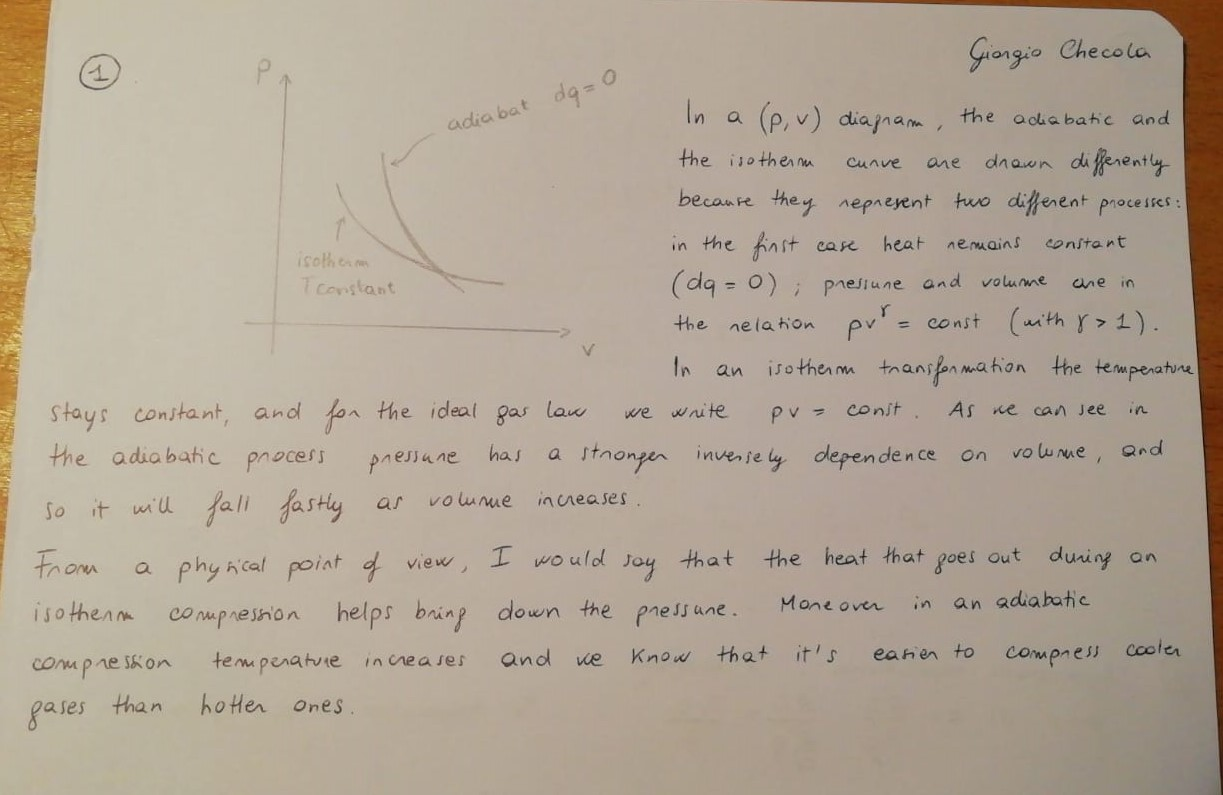
\includegraphics[width=150mm]{images/es1.JPEG}
\end{figure}
\begin{figure}[H]
	\centering 
	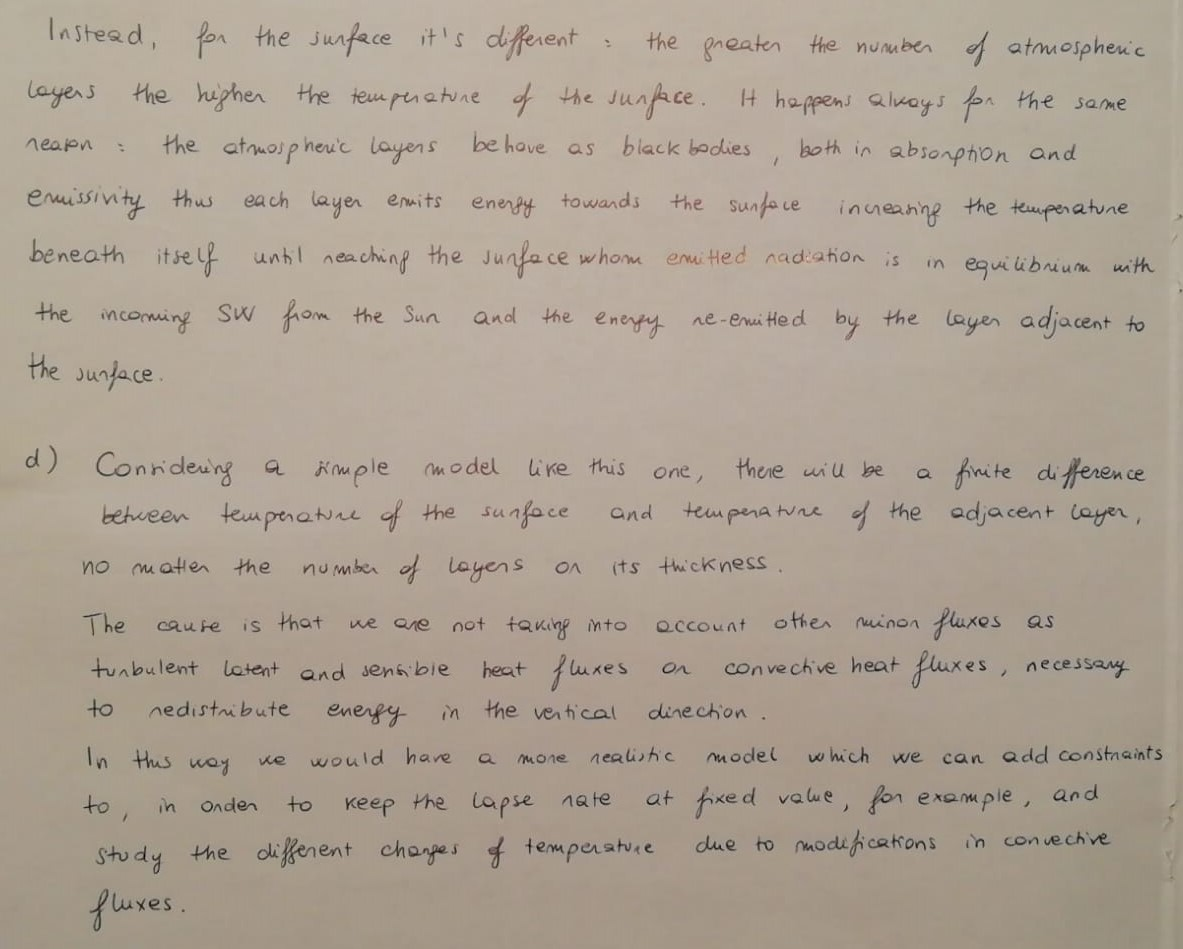
\includegraphics[width=150mm]{images/es1_1.JPEG}
\end{figure}
	
\subsection{Exercise 2}
\begin{figure}[H]
	\centering 
	
\includegraphics[width=150mm]{images/es0.PNG}
	
	\bigskip
	
	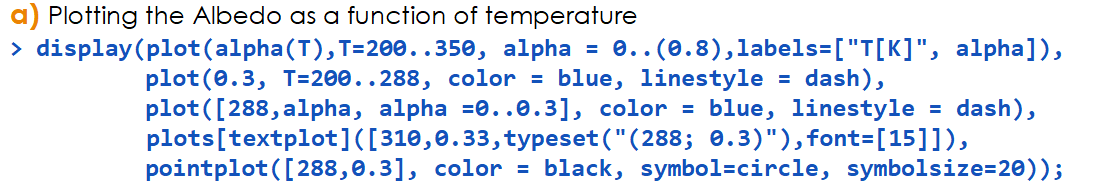
\includegraphics[width=150mm]{images/es2_0.PNG}
	
	\smallskip
	
	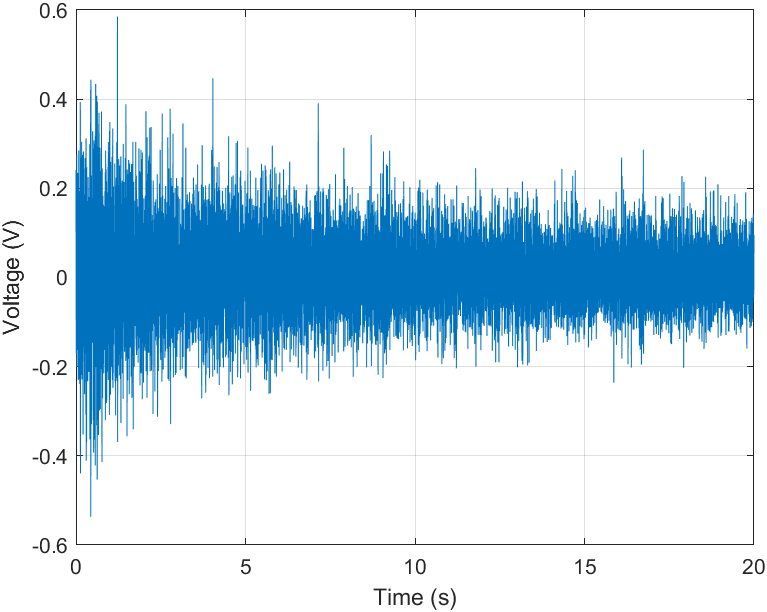
\includegraphics[width=75mm]{images/plot1.PNG}
	
	\bigskip
	
	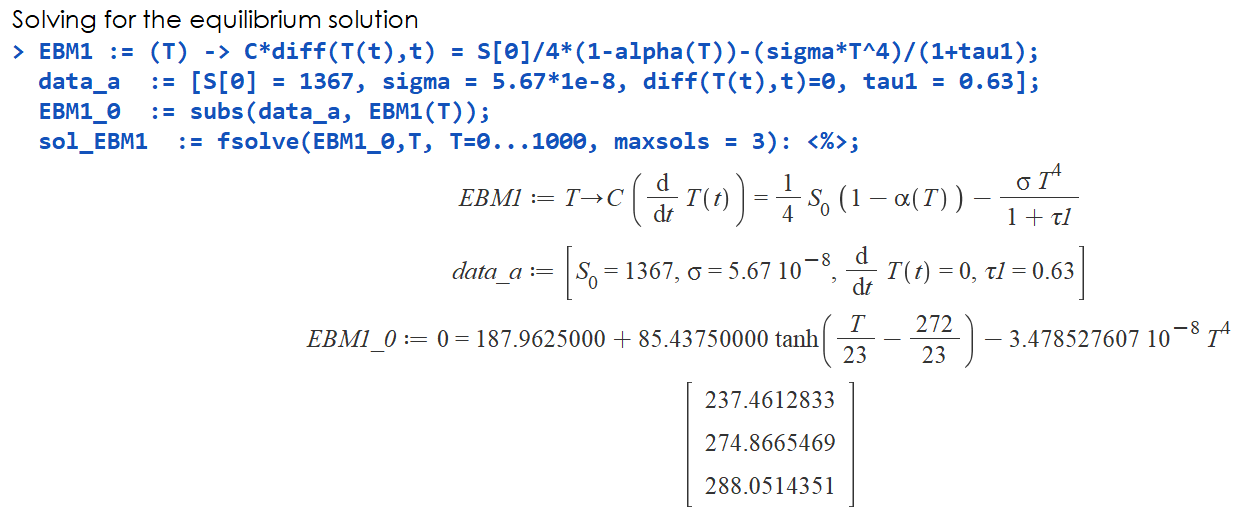
\includegraphics[width=150mm]{images/es2_1.PNG}

\end{figure}

\begin{figure}[H]
	\centering
	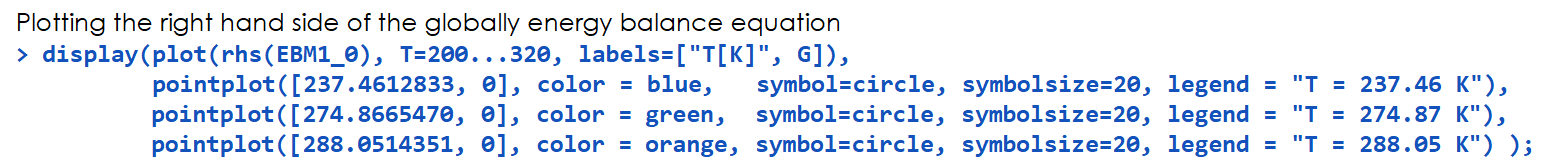
\includegraphics[width=150mm]{images/es2_2.PNG}
	
	\smallskip
	
	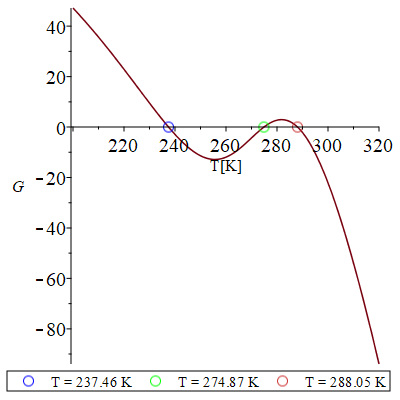
\includegraphics[width=75mm]{images/plot2.PNG}
	
	\smallskip
	
	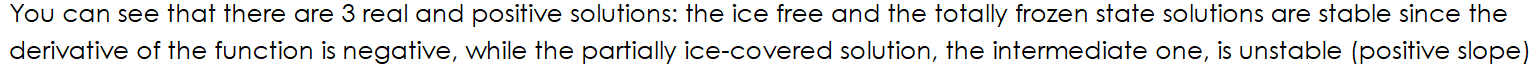
\includegraphics[width=150mm]{images/es2_3.PNG}
	
	\bigskip
	
	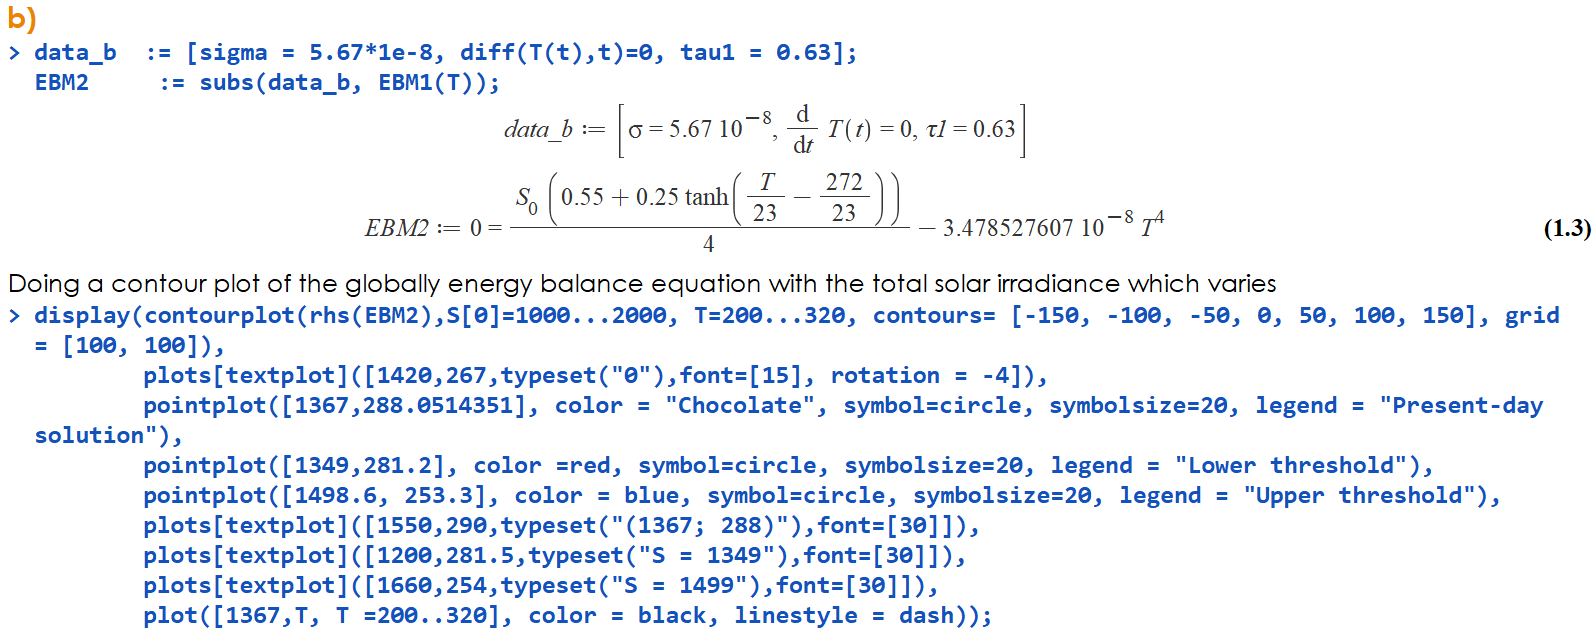
\includegraphics[width=150mm]{images/es2_4.PNG}
	
	\smallskip
	
	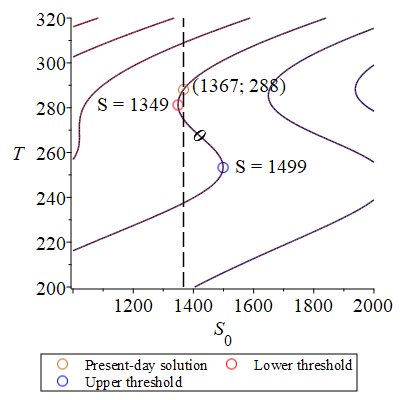
\includegraphics[width=75mm]{images/plot3.PNG}
\end{figure}	

\begin{figure}[H]
	\centering
	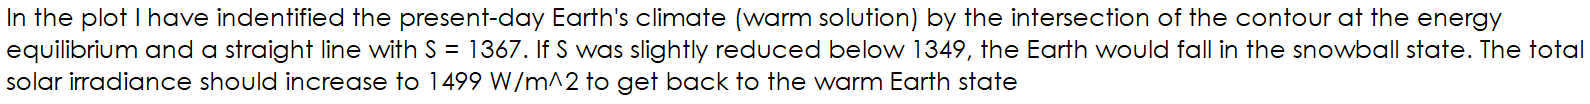
\includegraphics[width=150mm]{images/es2_5.PNG}
	
	\smallskip
	
	
\includegraphics[width=150mm]{images/es2_6.PNG}
	
	\smallskip
	
	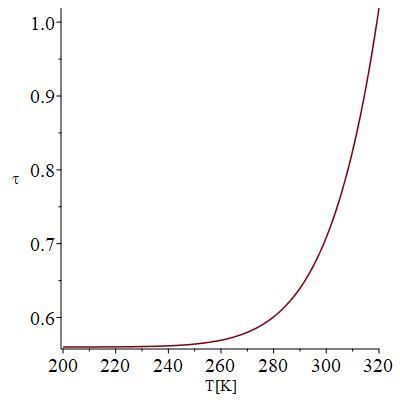
\includegraphics[width=75mm]{images/plot4.PNG}
	
	\bigskip
	
	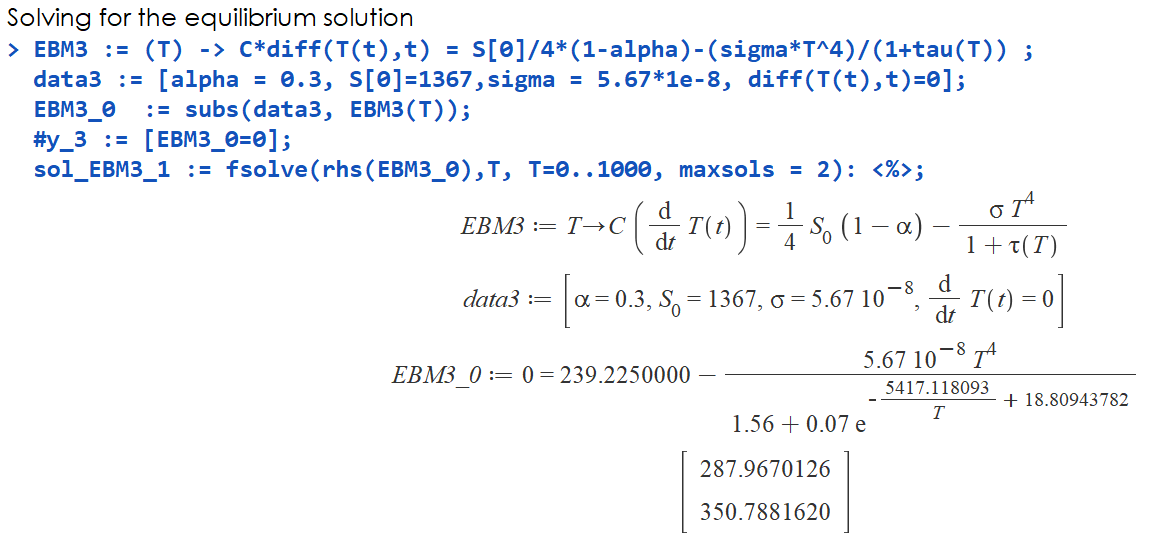
\includegraphics[width=150mm]{images/es2_7.PNG}
	
	\smallskip
	
	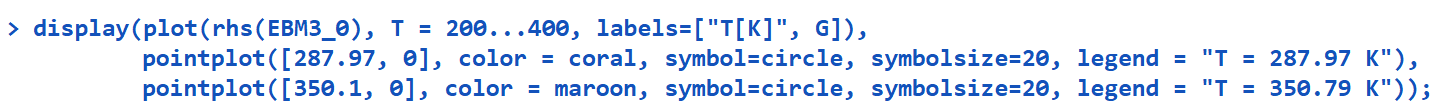
\includegraphics[width=150mm]{images/es2_8.PNG}
	
	\smallskip
	
	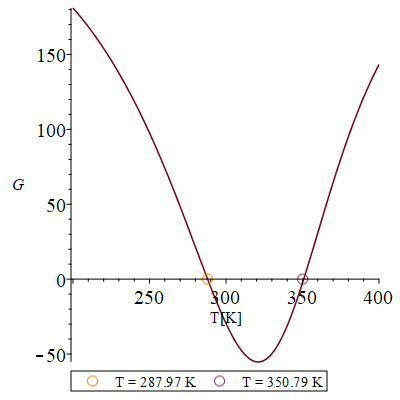
\includegraphics[width=75mm]{images/plot5.PNG}
\end{figure}

\begin{figure}[H]
	\centering
	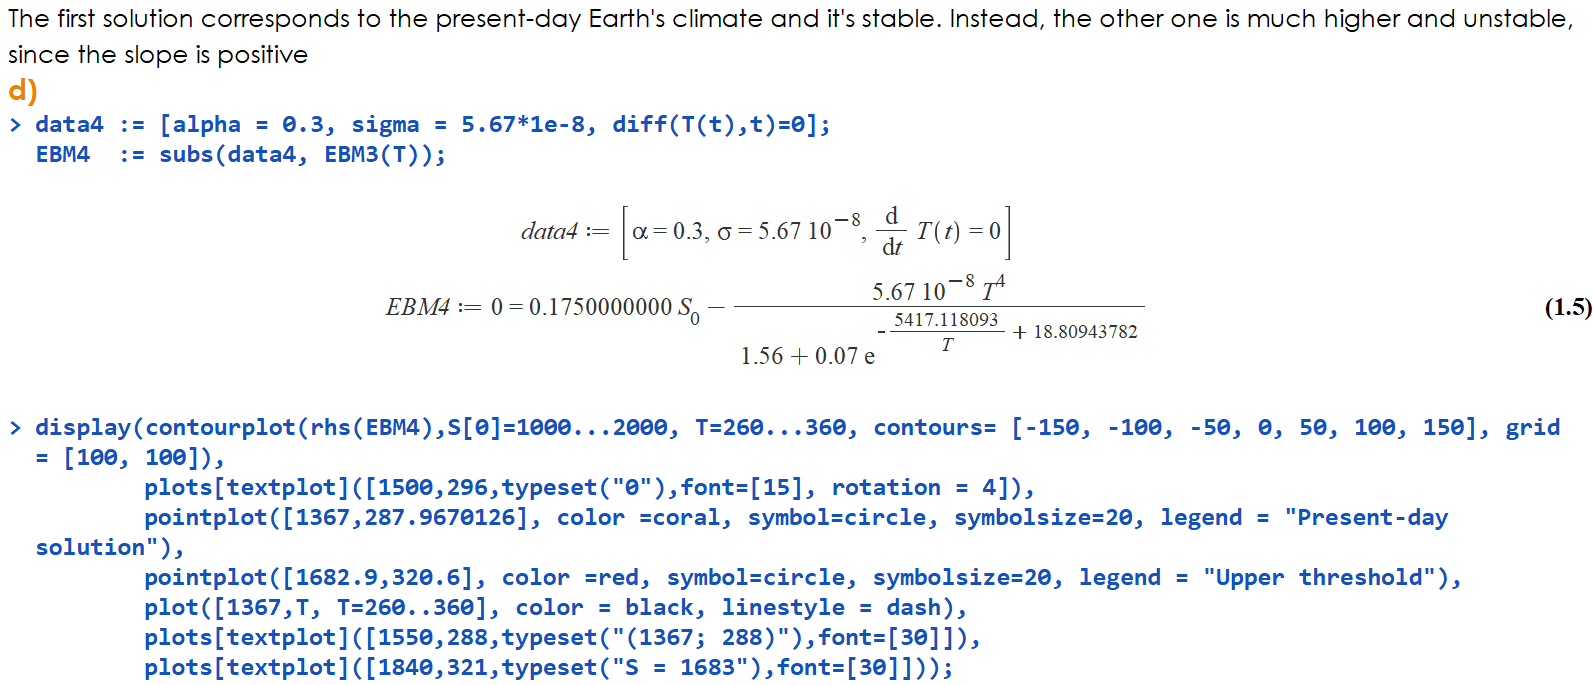
\includegraphics[width=150mm]{images/es2_9.PNG}
	
	\smallskip
	
	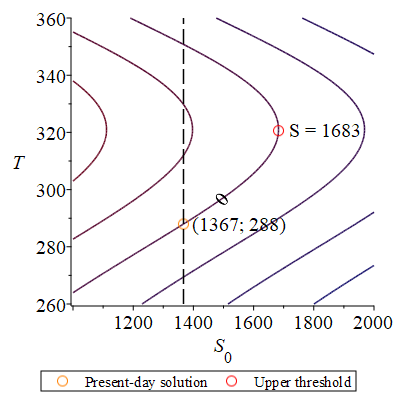
\includegraphics[width=75mm]{images/plot6.PNG}
	
	\smallskip
	
	
\includegraphics[width=150mm]{images/es2_10.PNG}
	
\end{figure}

\end{document}